\section{实验与分析}
\label{sec:evaluation}
\subsection{实验设计}
本文实现了单服务器与多服务器两种协议。我们根据数据库规模$\dbsize$、安全参数$\lambda$和查询次数$\querycount$来计算参数,以确保安全级别至少为$\lambda=128$,支持至少$\querycount=\sqrt{\dbsize}\log{\dbsize}$次查询(其中$\dbsize$为数据库中的记录数)。所有测试均在单线程环境中进行,并取10次运行结果的平均值。对于双服务器PIR协议,两个服务器的操作串行执行。我们对这些协议的离线阶段和在线阶段进行了测试,并考虑了存储成本。例如,Piano协议要求在线阶段缓存查询结果,这种存储开销也包含在存储成本中。数据传输时间不计入时间计算,但总通信量将详细说明。实验在配备16核Intel(R) Xeon(R) E-2288G CPU @ 3.70GHz和128GiB内存的服务器上进行。共进行了五个数据库的测试,数据库大小从256MiB到32GiB不等,但都由32字节的记录组成。

我们对本文提出的协议性能进行了全面评估,并与当前领先的双服务器PIR、单服务器PIR和可验证PIR协议进行了比较。由于本文的验证过程可以选择启用或禁用,我们测试了两种不同版本:一种是包含验证功能的版本,另一种是不包含验证功能的版本。在结果展示中,“本文(NV)”代表未包含验证过程的本文版本。在双服务器PIR方面,我们选取了DPF-PIR \cite{EC:GilIsh14}、TreePIR \cite{C:LazPap23}和APIR \cite{APIR}作为比较对象。对于单服务器协议,我们选取了SimplePIR \cite{SimplePIR}、VeriSimplePIR \cite{VeriSimplePIR}和Piano \cite{Piano}进行对比。其中,VeriSimplePIR和APIR是可验证PIR协议,能够确保对恶意服务器响应完整性的验证。而其他协议基于半诚实服务器的假设。

在测试过程中,我们主要关注两个问题:(i) 验证的成本是多少?(ii) 本文的协议相对于当前领先的PIR协议表现如何?

\begin{table*}[]
    \caption{双服务器PIR协议的对比}
    \label{tab:two-server-evaluation}
    \resizebox{\columnwidth}{!}{%
    \begin{tabular}{@{}lc|ccc|cccccc@{}}
        \toprule
                  & \multicolumn{1}{l|}{}     & \multicolumn{3}{c|}{离线} & \multicolumn{6}{c}{在线}                                                                                                                      \\ \midrule
                  & \multicolumn{1}{l|}{}     & 通信量(MiB)                     & 存储(MiB)                & 时间(s) & \multicolumn{2}{c|}{通信量(KiB)} & \multicolumn{4}{c}{时间(ms)}                                             \\
                  & \multicolumn{1}{l|}{}     &                              &                            &         & 下载                      & \multicolumn{1}{c|}{上传}  & Query & Answer   & Reconstruct & 共计    \\ \midrule
        本文     & \multirow{5}{*}{128 MiB} & 4.95                         & 9.21                       & 8.28    & 64.07                         & \multicolumn{1}{c|}{80.02}   & 0.04  & 0.09     & 0.02        & 0.15     \\
        本文(NV) &                           & 2.51                         & 4.64                       & 2.08    & 64.04                         & \multicolumn{1}{c|}{16.02}   & 0.03  & 0.06     & 0.00        & 0.09     \\
        DPF-PIR       &                           & 0.00                         & 0.00                       & 0.00    & 0.06                          & \multicolumn{1}{c|}{0.84}    & 0.02  & 45.10    & 0.00        & 45.12    \\
        TreePIR   &                           & 4.27                         & 4.88                       & 1.66    & 128.20                        & \multicolumn{1}{c|}{0.58}    & 0.62  & 0.72     & 0.00        & 1.35     \\
        APIR      &                           & 0.00                         & 0.00                       & 0.00    & 2980.00                       & \multicolumn{1}{c|}{0.50}    & 0.00  & 295.85   & 0.02        & 295.87   \\ \midrule
        本文     & \multirow{5}{*}{512 MiB} & 9.89                         & 18.42                      & 38.20   & 128.07                        & \multicolumn{1}{c|}{160.02}  & 0.09  & 0.25     & 0.04        & 0.37     \\
        本文(NV) &                           & 5.02                         & 9.28                       & 8.77    & 128.04                        & \multicolumn{1}{c|}{32.02}   & 0.05  & 0.15     & 0.00        & 0.21     \\
        DPF-PIR       &                           & 0.00                         & 0.00                       & 0.00    & 0.06                          & \multicolumn{1}{c|}{0.91}    & 0.03  & 185.91   & 0.00        & 185.94   \\
        TreePIR   &                           & 8.53                         & 9.75                       & 6.77    & 256.20                        & \multicolumn{1}{c|}{0.61}    & 1.26  & 1.60     & 0.00        & 2.85     \\
        APIR      &                           & 0.00                         & 0.00                       & 0.00    & 6472.00                       & \multicolumn{1}{c|}{1.00}    & 0.00  & 1231.91  & 0.02        & 1231.93  \\ \midrule
        本文     & \multirow{5}{*}{2 GiB}   & 20.28                        & 37.78                      & 166.70  & 256.07                        & \multicolumn{1}{c|}{320.02}  & 0.23  & 0.69     & 0.08        & 1.00     \\
        本文(NV) &                           & 10.28                        & 19.03                      & 36.31   & 256.04                        & \multicolumn{1}{c|}{64.02}   & 0.14  & 0.38     & 0.01        & 0.53     \\
        DPF-PIR       &                           & 0.00                         & 0.00                       & 0.00    & 0.06                          & \multicolumn{1}{c|}{0.98}    & 0.03  & 710.96   & 0.00        & 710.99   \\
        TreePIR   &                           & 17.50                        & 20.00                      & 28.48   & 512.20                        & \multicolumn{1}{c|}{0.64}    & 2.65  & 3.52     & 0.00        & 6.17     \\
        APIR      &                           & 0.00                         & 0.00                       & 0.00    & 13968.00                      & \multicolumn{1}{c|}{2.00}    & 0.01  & 5247.01  & 0.02        & 5247.03  \\ \midrule
        本文     & \multirow{5}{*}{8 GiB}   & 41.56                        & 77.44                      & 827.72  & 512.07                        & \multicolumn{1}{c|}{640.02}  & 0.49  & 2.07     & 0.16        & 2.72     \\
        本文(NV) &                           & 21.06                        & 39.00                      & 243.44  & 512.04                        & \multicolumn{1}{c|}{128.02}  & 0.33  & 1.12     & 0.02        & 1.47     \\
        DPF-PIR       &                           & 0.00                         & 0.00                       & 0.00    & 0.06                          & \multicolumn{1}{c|}{1.05}    & 0.03  & 2832.52  & 0.00        & 2832.55  \\
        TreePIR   &                           & 35.88                        & 41.00                      & 123.42  & 1024.20                       & \multicolumn{1}{c|}{0.67}    & 5.52  & 7.69     & 0.00        & 13.20    \\
        APIR      &                           & -                            & -                          & -       & -                             & \multicolumn{1}{c|}{-}       & -     & -        & -           & -        \\ \midrule
        本文     & \multirow{5}{*}{32 GiB}  & 85.13                        & 158.63                     & 3838.58 & 1024.07                       & \multicolumn{1}{c|}{1280.02} & 1.30  & 4.73     & 0.53        & 6.56     \\
        本文(NV) &                           & 43.13                        & 79.88                      & 1311.07 & 1024.04                       & \multicolumn{1}{c|}{256.02}  & 1.11  & 2.50     & 0.04        & 3.65     \\
        DPF-PIR       &                           & 0.00                         & 0.00                       & 0.00    & 0.06                          & \multicolumn{1}{c|}{1.12}    & 0.03  & 11413.70 & 0.00        & 11413.73 \\
        TreePIR   &                           & 73.50                        & 84.00                      & 510.92  & 2048.20                       & \multicolumn{1}{c|}{0.70}    & 11.33 & 16.86    & 0.00        & 28.19    \\
        APIR      &                           & -                            & -                          & -       & -                             & \multicolumn{1}{c|}{-}       & -     & -        & -           & -        \\ \bottomrule
    \end{tabular}
    }
\end{table*}

\begin{table*}[]
    \caption{单服务器PIR协议的对比}
    \label{tab:single-server-evaluation}
    \resizebox{\columnwidth}{!}{%
    \begin{tabular}{@{}cc|ccc|cccccc@{}}
        \toprule
                      &                           & \multicolumn{3}{c|}{离线} & \multicolumn{6}{c}{在线}                                                                                                                    \\ \midrule
                      &                           & 通信量(MiB)                     & 存储(MiB)                & 时间(s)  & \multicolumn{2}{c|}{通信量(KiB)} & \multicolumn{4}{c}{时间(ms)}                                          \\
                      &                           &                              &                            &          & 下载                      & \multicolumn{1}{c|}{上传}  & Query  & Answer & Reconstruct & 总计  \\ \midrule
        本文         & \multirow{5}{*}{128 MiB} & 128.00                       & 23.89                      & 21.43    & 0.06                          & \multicolumn{1}{c|}{72.02}   & 0.04   & 0.05   & 0.00        & 0.09   \\
        本文(NV)     &                           & 128.00                       & 14.10                      & 10.02    & 0.03                          & \multicolumn{1}{c|}{8.01}    & 0.03   & 0.02   & 0.00        & 0.05   \\
        SimplePIR     &                           & 41.00                        & 41.00                      & 20.79    & 41.00                         & \multicolumn{1}{c|}{41.00}   & 14.26  & 9.49   & 2.20        & 25.95  \\
        VeriSimplePIR &                           & 231.17                       & 101.25                     & 285.06   & 50.63                         & \multicolumn{1}{c|}{50.57}   & 25.99  & 15.40  & 8.52        & 49.91  \\
        Piano         &                           & 128.00                       & 20.92                      & 42.29    & 63.99                         & \multicolumn{1}{c|}{8.02}    & 0.54   & 0.16   & 0.00        & 0.70   \\ \midrule
        本文         & \multirow{5}{*}{512 MiB} & 512.00                       & 49.94                      & 90.81    & 0.06                          & \multicolumn{1}{c|}{144.02}  & 0.08   & 0.15   & 0.00        & 0.23   \\
        本文(NV)     &                           & 512.00                       & 29.61                      & 42.26    & 0.03                          & \multicolumn{1}{c|}{16.01}   & 0.05   & 0.05   & 0.00        & 0.10   \\
        SimplePIR     &                           & 84.00                        & 84.00                      & 89.42    & 84.00                         & \multicolumn{1}{c|}{84.00}   & 29.38  & 42.12  & 4.33        & 75.83  \\
        VeriSimplePIR &                           & 488.43                       & 212.50                     & 1231.67  & 106.25                        & \multicolumn{1}{c|}{106.02}  & 53.81  & 66.14  & 17.65       & 137.59 \\
        Piano         &                           & 512.00                       & 43.46                      & 245.58   & 127.99                        & \multicolumn{1}{c|}{16.02}   & 1.04   & 0.30   & 0.00        & 1.34   \\ \midrule
        本文         & \multirow{5}{*}{2 GiB}   & 2048.00                      & 108.68                     & 392.20   & 0.06                          & \multicolumn{1}{c|}{288.02}  & 0.22   & 0.52   & 0.00        & 0.73   \\
        本文(NV)     &                           & 2048.00                      & 64.67                      & 176.90   & 0.03                          & \multicolumn{1}{c|}{32.01}   & 0.14   & 0.14   & 0.00        & 0.28   \\
        SimplePIR     &                           & 169.00                       & 169.00                     & 363.72   & 169.00                        & \multicolumn{1}{c|}{169.00}  & 58.93  & 161.94 & 8.52        & 229.39 \\
        VeriSimplePIR &                           & 984.05                       & 424.75                     & 4864.49  & 212.38                        & \multicolumn{1}{c|}{212.16}  & 107.59 & 263.29 & 34.94       & 405.83 \\
        Piano         &                           & 2048.00                      & 93.93                      & 759.98   & 255.99                        & \multicolumn{1}{c|}{32.02}   & 1.91   & 0.55   & 0.00        & 2.46   \\ \midrule
        本文         & \multirow{5}{*}{8 GiB}   & 8192.00                      & 227.48                     & 1620.31  & 0.06                          & \multicolumn{1}{c|}{576.02}  & 0.52   & 1.46   & 0.00        & 1.98   \\
        本文(NV)     &                           & 8192.00                      & 135.66                     & 783.71   & 0.03                          & \multicolumn{1}{c|}{64.01}   & 0.45   & 0.46   & 0.00        & 0.91   \\
        SimplePIR     &                           & 344.00                       & 344.00                     & 1612.35  & 344.00                        & \multicolumn{1}{c|}{344.00}  & 118.35 & 684.98 & 18.21       & 821.54 \\
        VeriSimplePIR &                           & -                            & -                          & -        & -                             & \multicolumn{1}{c|}{-}       & -      & -      & -           & -      \\
        Piano         &                           & 8192.00                      & 196.20                     & 3319.58  & 511.99                        & \multicolumn{1}{c|}{64.02}   & 3.82   & 1.13   & 0.00        & 4.95   \\ \midrule
        本文         & \multirow{5}{*}{32 GiB}  & 32768.00                     & 475.07                     & 6811.69  & 0.06                          & \multicolumn{1}{c|}{1152.02} & 1.17   & 3.29   & 0.00        & 4.46   \\
        本文(NV)     &                           & 32768.00                     & 283.87                     & 3117.62  & 0.03                          & \multicolumn{1}{c|}{128.01}  & 0.71   & 0.94   & 0.00        & 1.66   \\
        SimplePIR     &                           & -                            & -                          & -        & -                             & \multicolumn{1}{c|}{-}       & -      & -      & -           & -      \\
        VeriSimplePIR &                           & -                            & -                          & -        & -                             & \multicolumn{1}{c|}{-}       & -      & -      & -           & -      \\
        Piano         &                           & 32768.00                     & 409.08                     & 13490.68 & 1023.99                       & \multicolumn{1}{c|}{128.02}  & 7.64   & 2.36   & 0.00        & 10.00  \\ \bottomrule
    \end{tabular}%
    }
\end{table*}
\subsection{结果分析}

\paragraph{双服务器协议}
双服务器PIR协议的基准测试结果如表 \ref{tab:two-server-evaluation} 所示。DPF-PIR和APIR协议没有采用离线-在线模型。在数据库大于8 GiB时,APIR会消耗超过128 GiB的内存,无法完成测试。比较本文两个版本,可以明显看出,验证功能会导致离线计算增加约3-4倍,在线计算增加2倍,通信和存储成本增加1倍。

在这些协议中,本文的协议在在线计算方面超越了当前领先的亚线性协议TreePIR~\cite{C:LazPap23},且总体通信量更小。优越的性能主要源于协议简化了查询构造以及对虚构查询的消除,在线阶段不再需要昂贵的wPPRF和虚构查询。离线阶段,本文协议通过使用一个主密钥表示集合,通信成本稍低,但因为缺少AVX指令的实现,计算成本稍高。

DPF-PIR~\cite{EC:GilIsh14} 是一个线性PIR协议,这意味着其在线计算时间随着数据库大小线性增长。对于32 GiB的数据库,DPF-PIR执行一次查询需要超过10秒。而相比之下,我们的协议在执行相同操作时只需不到10毫秒。这一显著的性能差异强调了使用亚线性PIR协议的重要性,尤其是在处理大规模数据库时,它能显著提高查询效率,减少计算时间。

APIR \cite{APIR} 是目前领先的双服务器可验证PIR协议。本文的协议在所有数据库大小中均在计算效率上超越了APIR。此外,基于Merkle证明的APIR需要对数据库进行预处理,导致数据库大小显著增加。这使其受限于内存不足问题,无法在大于8 GiB的数据库上运行。

\paragraph{单服务器协议}
单服务器PIR协议的测试结果如表 \ref{tab:single-server-evaluation} 所示。VeriSimplePIR在数据库大于8GiB时以及SimplePIR在数据库大于32GiB时消耗超过128 GiB的内存,无法完成测试。

Piano~\cite{Piano} 是当前最先进的单服务器亚线性协议。Piano要求服务器计算$\sqrt{\dbsize}$个答案以隐藏被查询的索引,增加了计算和通信成本。因此,本文的协议在计算和通信上均优于Piano:在线计算速度提高的同时,在线上传量相同,但在线下载量显著减少。

在离线阶段,Piano和本文协议都采用将数据库流式传输到客户端的策略,通信成本类似。理论上,这两个协议在离线计算和存储成本上相似。表中的差异主要归因于实现细节。

与线性单服务器PIR协议SimplePIR~\cite{SimplePIR}相比,本文协议在在线计算上显示出了显著的改进。SimplePIR需要线性时间计算答案,而本文协议仅需要亚线性计算。

与领先的单服务器可验证PIR协议VeriSimplePIR~\cite{VeriSimplePIR}相比,本文协议的在线上传量略大,但在线下载量却小得多,在线计算时间表现出类似SimplePIR的改进。表中有两个有趣的点:首先,SimplePIR和VeriSimplePIR导致了相当大的数据库膨胀,这意味着它们对服务器RAM提出了显著的挑战。其次,SimplePIR和VeriSimplePIR的客户端存储成本实际上高于本文提出的协议。

\paragraph{经济成本}
为了展示本文协议在实际场景中的实用性,我们在图 \ref{fig:single-server-cost} 中提供了本文协议和其他协议的经济成本估算。我们以客户端直接下载并存储数据库为基准,图中的数据以相对于该基准协议的成本比例显示。成本是基于AWS的定价\footnote{每GiB下载费用为0.05美元,每GiB数据存储在EBS gp3上的费用为0.08美元,c7a.2xlarge实例的每小时CPU费用为0.41美元。},对应之前实验中的2 GiB和8 GiB数据库计算的。我们假设客户端每月运行一定数量的查询,并且至少运行一次完整的离线阶段。由于SimplePIR和VeriSimplePIR的离线计算与客户端无关,因此离线计算成本不包含在内。

从之前的对比中,我们可以看到本文协议的在线上传量略大,但在线下载量却低得多。因此,本文协议在成本方面非常具有竞争力。当客户端每月运行超过$2^{12}$次查询时,本文协议比SimplePIR更具成本效益,并且在查询次数少于$2^{18}$时,本文协议的成本仍然低于直接存储数据库的协议。当数据库规模增大时,本文协议的优势保持到了更大的查询规模。这一结果清楚地表明,本文协议是一种在实际场景中,尤其是在客户端存储资源有限的情况下,提供PIR服务的可行方案。

\begin{figure*}
    \begin{subfigure}{0.5\textwidth}
        \centering
        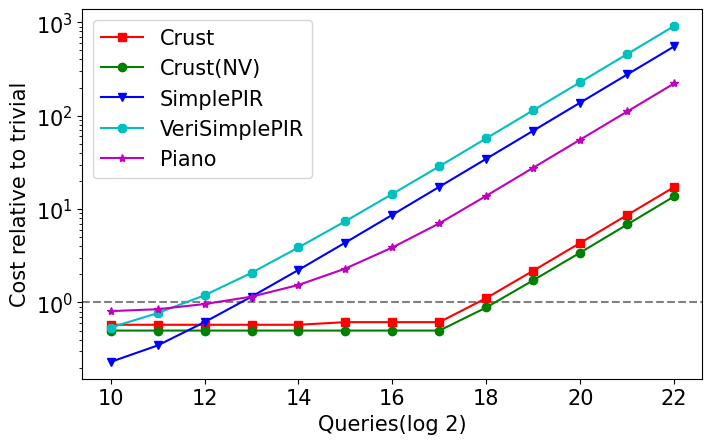
\includegraphics[width=0.8\linewidth]{figure/cost_2gb.png}
        \caption{2 GiB}
    \end{subfigure}%
    \begin{subfigure}{0.5\textwidth}
        \centering
        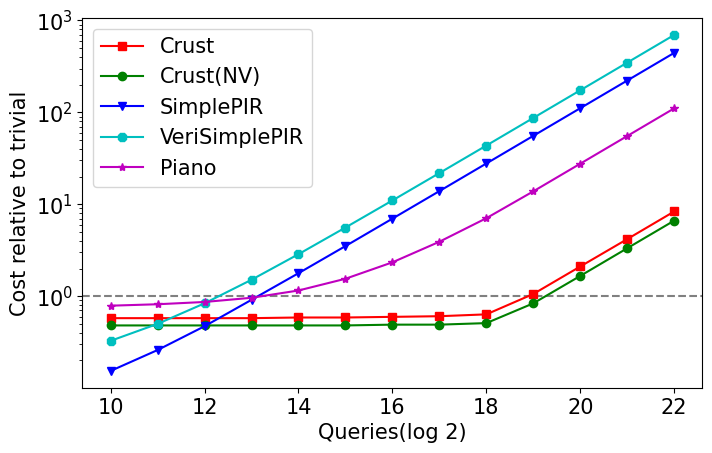
\includegraphics[width=0.8\linewidth]{figure/cost_8gb.png}
        \caption{8 GiB}
    \end{subfigure}%
    \caption{单服务器PIR协议在经济成本方面的对比}
    \label{fig:single-server-cost}
\end{figure*}